\chapter{Platform deployment tests, and results}\label{H:platformDeploymentAndDemonstrations}

In order to demonstrate that the LiveMediaStreamer is a suitable tool to be used as the core framework of a cloud real-time media production platform it is required to test how it performs over the cloud.

\section{Platform deployment}

In order to demonstrate how LMS fits the project requirements two scenarios, with different complexity, are deployed.

\begin{itemize}
\item Isolated deployments \hfill

The main goal of this deployment is to demonstrate how LMS performs inside a Docker container by comparing its performance in the same OS but without running inside a container (i.e.: system installation).

In this scenario LMS is configured to act as a transcoder service. This means applying one pipeline per stream type (i.e.: one video and one audio paths).

\item Generic deployment scenario \hfill

This scenario aims to showcase a suitable and as much generic as possible cloud real-time media production scenario. LMS is configured to receive eight streams (i.e.: four audio and four video streams), mix them and transmit them through RTP/RTSP. 
\end{itemize}

The environment where the deployments are done is composed of two laptops. The LMS container and the Collectd client container are deployed in laptop described in Table \ref{T:dec}. The second laptop is a Dual-Core PC with the Graphite container running. Note that the first laptop described has the highest computational cost because all the audio and video processing is done in. The second laptop only stores the statistics, displays the Graphite graphs in a browser, plays the LMS's output streams and transmits a video source (2 Mbps H.264 encoded video stream at 25 fps and at 1280x720 pixels resolution) as input for the LMS.

\begin{table}[htb]
\caption{Deployment environment characteristics}
\begin{center}
\begin{tabular}{|c|c|}
\hline
{\bf Parameter} & {\bf Value} \\ \hline \hline
Hardware type        & Sony VAIO laptop \\ \hline
CPU        & Intel core i7-3632QM at 2.20 GHz  \\ \hline
RAM        & 6 GB (4 + 2) DDR3 \\ \hline
Operating system        & XUbuntu 14.04 - 64 bits (x86 64)  \\ \hline
Kernel version        & 3.13.0-55-generic  \\ \hline
Docker version        & 1.6.8  \\ \hline
\end{tabular}
\label{T:dec}
\end{center}
\end{table}

As seen, the deployment has not been carried out in any type of specific server or high performance cluster environment. The main goal is to demonstrate flexibility on the deployment (i.e.: in a laptop) and portability of the platform (not only the cloud itself). All of these characteristics are achieved thanks to the performance of the platform itself and the LMS (the core).

Note that all tests have been carried out in a 1 Gbps local area network with a router with both laptops connected (see Figure \ref{F:idsc} and Figure \ref{F:gdsc}). The measurements have been carried out during 10 minutes and a second of granularity.

\subsection{Isolated deployments}

This section compares the performance of the LMS installed on system (i.e.: in the host OS) and the same LMS inside a container. A C/C++ script has been developed, which configures the LMS framework as shown in Figure \ref{F:idsc}. Moreover, in order to test the performance, the pipeline metrics are logged once per second (i.e.: pipeline losses and delay) and gathered by a Collectd client container properly configured. Then the Collectd client sends the data to the Graphite container. Check Appendix \ref{ANX:dockerFiles} section \ref{ANX:collectdTailFiles2} to see an example of how the logging and collecting is implemented for these demonstrations. 

\begin{figure}[!htb]
\begin{center}
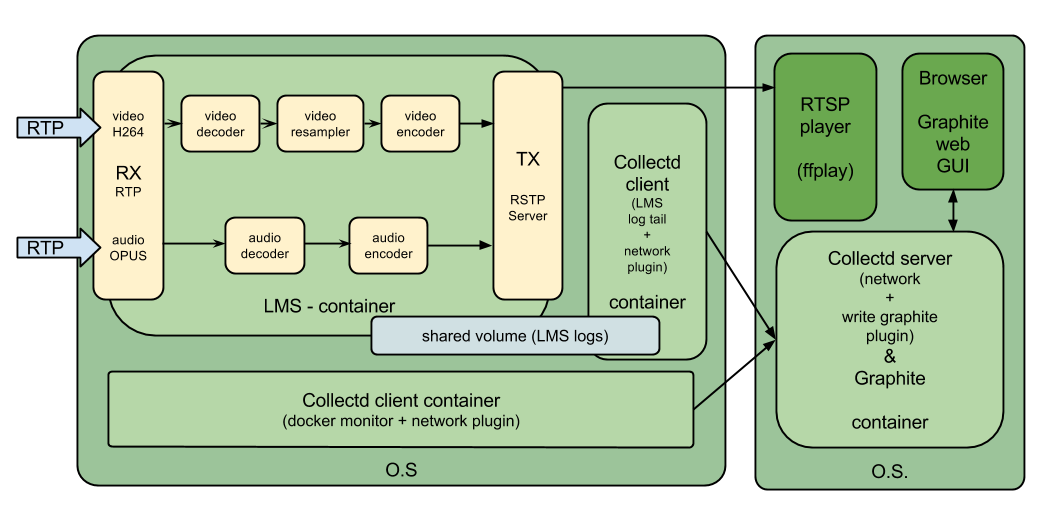
\includegraphics[width=0.95\textwidth]{./images/isolatedScenario.png}
\caption{Configuration of the scenario for the isolated deployments}
\label{F:idsc}
\end{center}
\end{figure}

The Collectd client container, which reads from the folder where the LMS is logging its metrics, uses the \texttt{tail} plugin (previously explained in Chapter \ref{G:monitoringLayer}) with specific regular expressions in order to parse the metrics from the LMS logs.

Both isolated scenarios are the same but one is running the LMS on the system and the other is running the same configured LMS but containerized. The second OS is the one which runs the Docker container with the Collectd+Graphite tools. Moreover, this OS acts as the receiver of the transcoded streams through the RTSP protocol and also acts as the transmitter of the source stream.

Figure \ref{F:isoCPU} shows the results. These are mainly focused on the pipeline performance metrics (i.e.: internal LMS performance). The figure describes the CPU usage gathered at the Collectd client side and presented for the Graphite web GUI for both isolated scenarios. Regarding system installation the CPU average usage of the averages given by Graphite is around 4,015\% and around 4,111\% for the containerized one. So, there is not so difference about running system installation or the same application containerized.

\begin{figure}[!htb]
  \begin{center}
    \begin{subfigmatrix}{2}
      \subfigure[System installation]
         {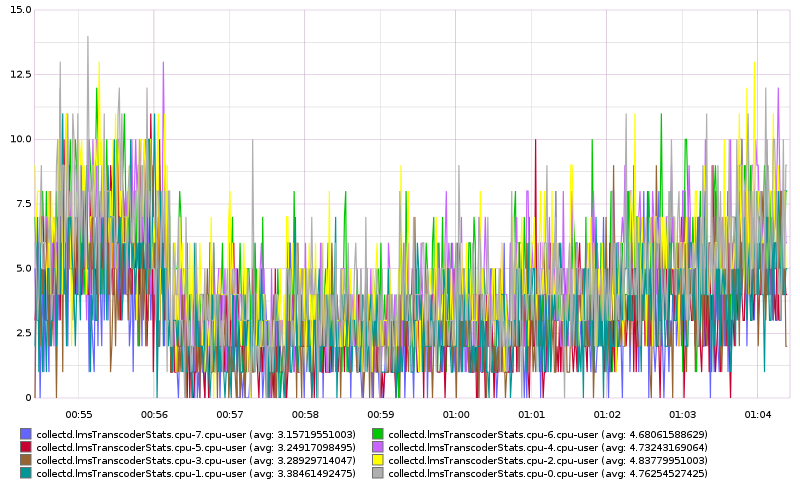
\includegraphics{./images/testStats/testStatsOS/8cpuIdleAVG.png}\label{SF:S1}} 
      \subfigure[Containerized]
         {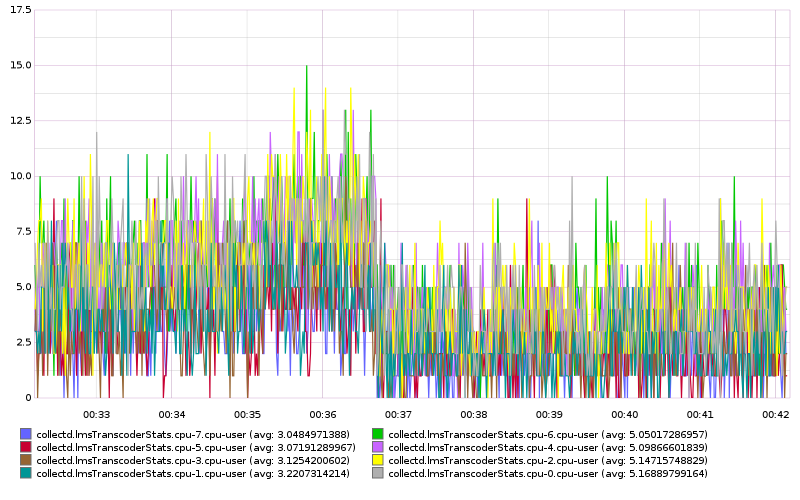
\includegraphics{./images/testStats/testStatsDocker/8cpuIdleAVG.png}\label{SF:S2}} 
    \end{subfigmatrix}
    \caption{Isolated scenarios - CPU usage}
    \label{F:isoCPU}
  \end{center}
\end{figure}

Figure \ref{F:isoappt} illustrates the average pipeline delay introduced by the LMS system, which in both video and audio cases is almost the same. Regarding video, system installation reaches an average of 216,8 milliseconds and the containerized case reaches an average of 215,9 milliseconds. Regarding audio, system installation reaches an average of 25,6 milliseconds and the containerized reaches an average of 25,2 milliseconds.

\begin{figure}[!htb]
  \begin{center}
    \begin{subfigmatrix}{2}
      \subfigure[System installation - Video path]
         {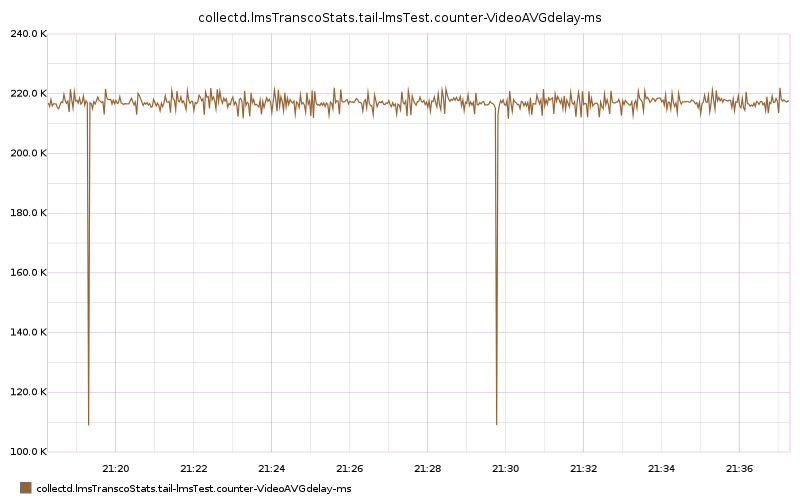
\includegraphics{./images/testStats/testStatsOS/vAVGdelayMS.png}\label{SF:S3}} 
      \subfigure[Containerized - Video path]
         {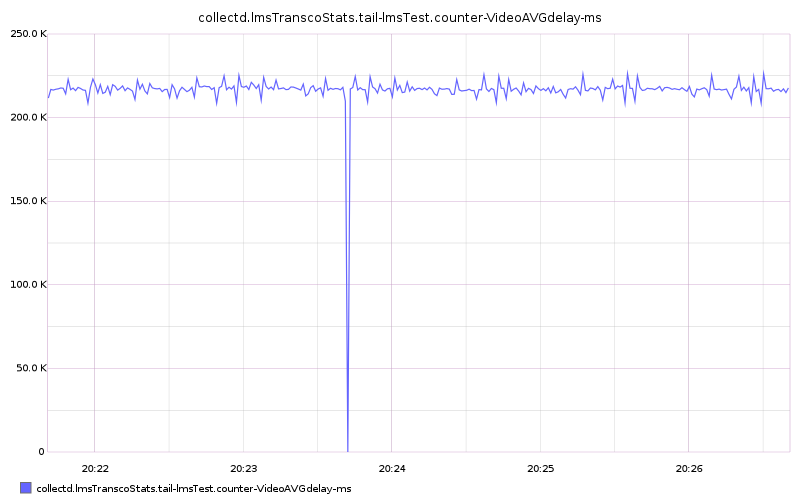
\includegraphics{./images/testStats/testStatsDocker/vAVGdelayMS.png}\label{SF:S4}} 
      \subfigure[System installation - Audio path]
         {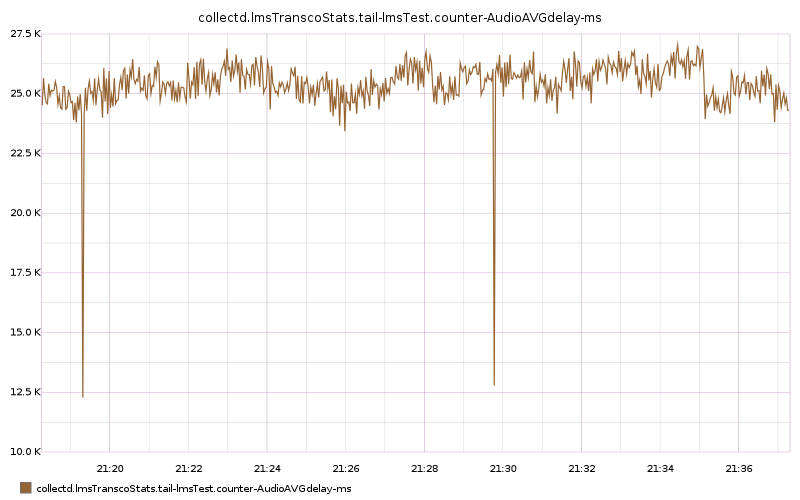
\includegraphics{./images/testStats/testStatsOS/aAVGdelayMS.png}\label{SF:S3}} 
      \subfigure[Containerized - Audio path]
         {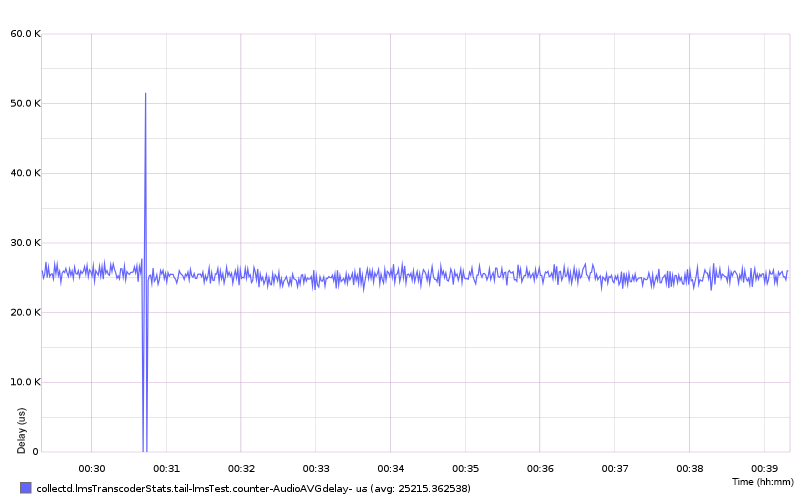
\includegraphics{./images/testStats/testStatsDocker/aAVGdelayMS.png}\label{SF:S4}}
    \end{subfigmatrix}
    \caption{Isolated scenarios - average pipeline processing time}
    \label{F:isoappt}
  \end{center}
\end{figure}



\begin{figure}[!htb]
  \begin{center}
    \begin{subfigmatrix}{2}
      \subfigure[System installation - Video path]
         {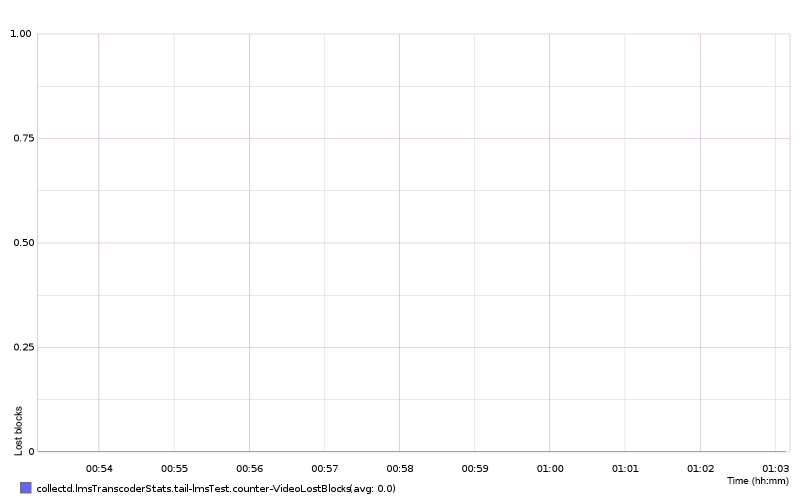
\includegraphics{./images/testStats/testStatsOS/vLostBlocs.png}\label{SF:S3}} 
      \subfigure[Containerized - Video path]
         {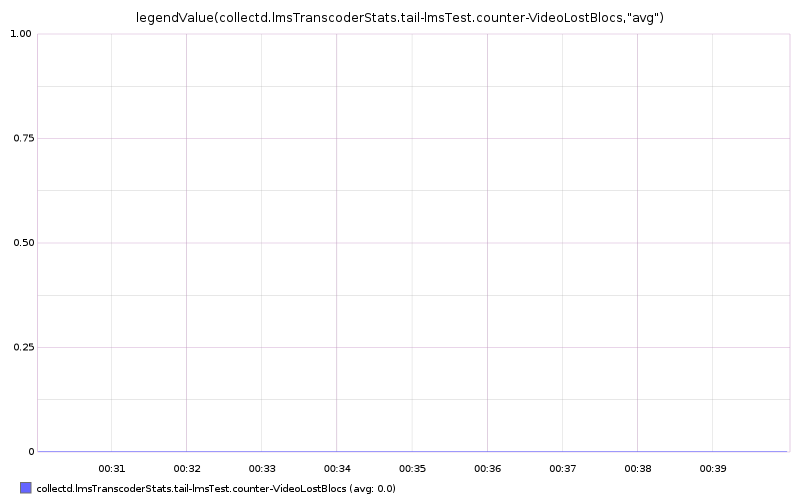
\includegraphics{./images/testStats/testStatsDocker/vLostBlocs.png}\label{SF:S4}} 
      \subfigure[System installation - Audio path]
         {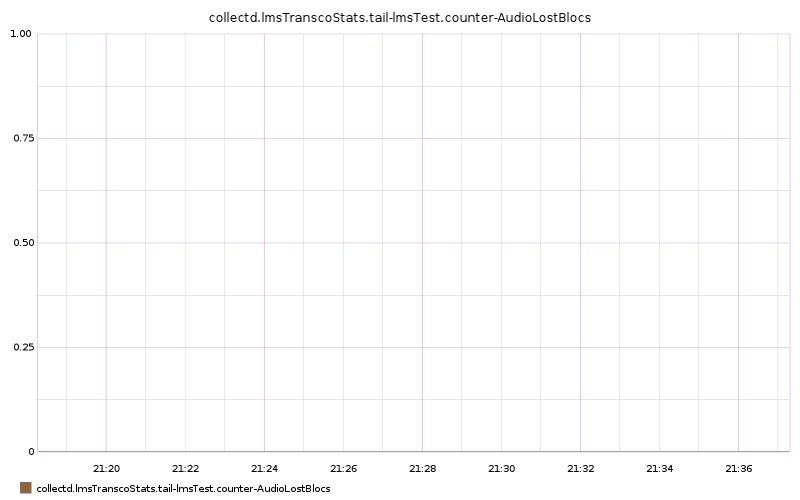
\includegraphics{./images/testStats/testStatsOS/aLostBlocs.png}\label{SF:S3}} 
      \subfigure[Containerized - Audio path]
         {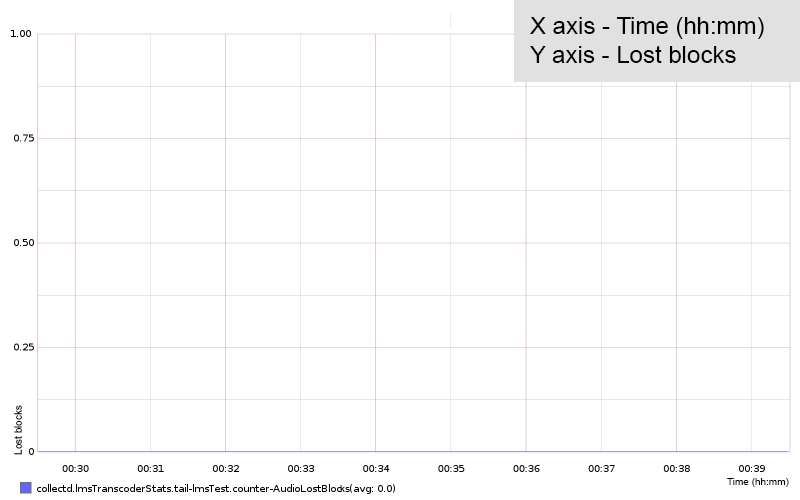
\includegraphics{./images/testStats/testStatsDocker/aLostBlocs.png}\label{SF:S4}}
    \end{subfigmatrix}
    \caption{Isolated scenarios - pipeline accumulated lost blocks}
    \label{F:isoaplb}
  \end{center}
\end{figure} 

\vbox{Regarding pipeline losses, as shown in Figure \ref{F:isoaplb}, both pipelines within both system installation and containerized scenarios do not introduce any data loss. Therefore, LMS is a good option to work with, not only on system installation but also in a containerized environment in order to be a portable service over a cloud infrastructure.}

\subsection{Generic scenario deployment}

This last scenario is a generic and basic example demonstration of audio and video production in a cloud environment. Figure \ref{F:gdsc} illustrates how the scenario is configured.

\begin{figure}[htb]
\begin{center}
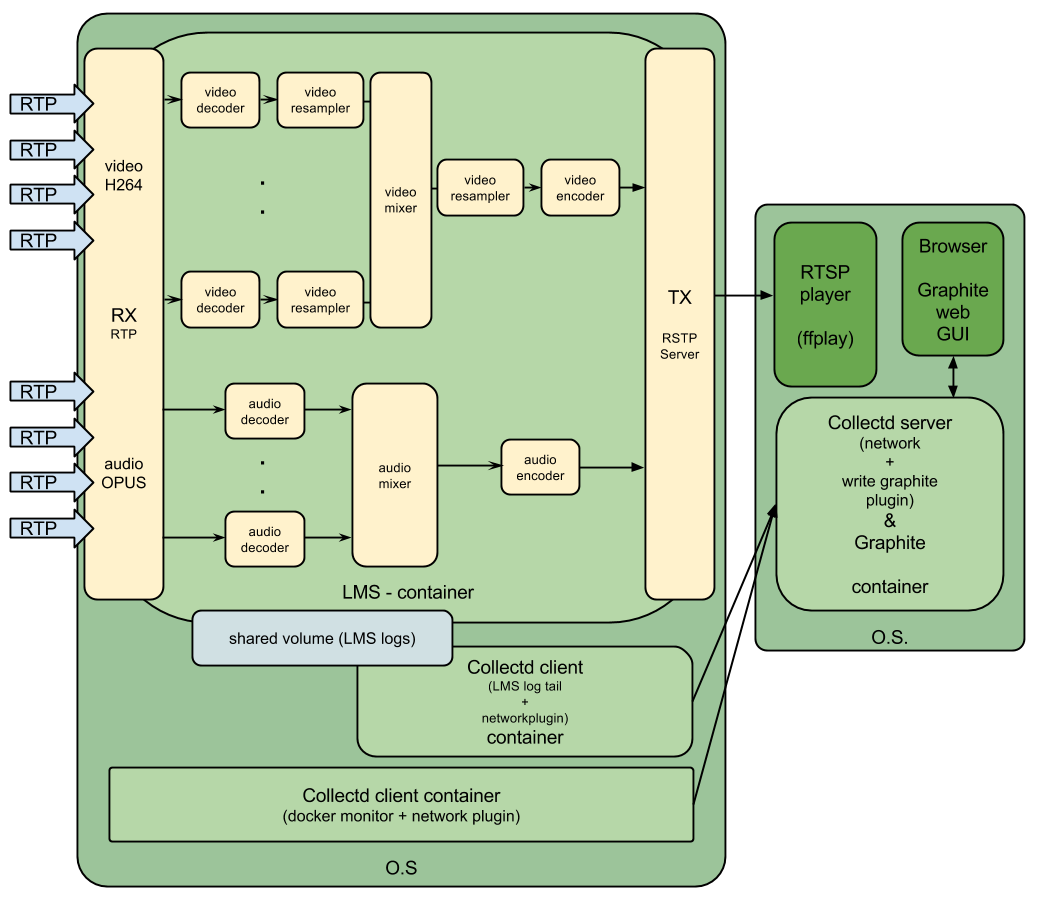
\includegraphics[width=0.95\textwidth]{./images/genericScenario.png}
\caption{Configuration of the scenario for the generic deployment}
\label{F:gdsc}
\end{center}
\end{figure}

This demonstration is quite similar to the previous but this time LMS is only configured and running inside a container. This LMS configuration is also a C/C++ script which configures the framework, as shown in Figure \ref{F:gdsc}, inside the LMS container, specifically.

In this case what is deployed is an audio and video mixer which receives four audio streams and four video streams encoded with OPUS and H264 codecs, respectively, which are streamed through its standard RTP encapsulation (i.e.: specific payload headers).

Regarding the audio mixing, all input streams are mixed using the logarithmic mixing algorithm in order to not saturate the signal of the resulting audio stream. Regarding the video mixing, the HD inputs (at 1280x720 pixels resolution) are mixed as shown in Figure \ref{F:outVMix}. All video inputs are resized (through the pre-resampler filter to the video mixer, see Figure \ref{F:gdsc}) to half of its size in order to fit into a resulting HD video stream as shown in Figure \ref{F:gdsc}.

\begin{figure}[!htb]
\begin{center}
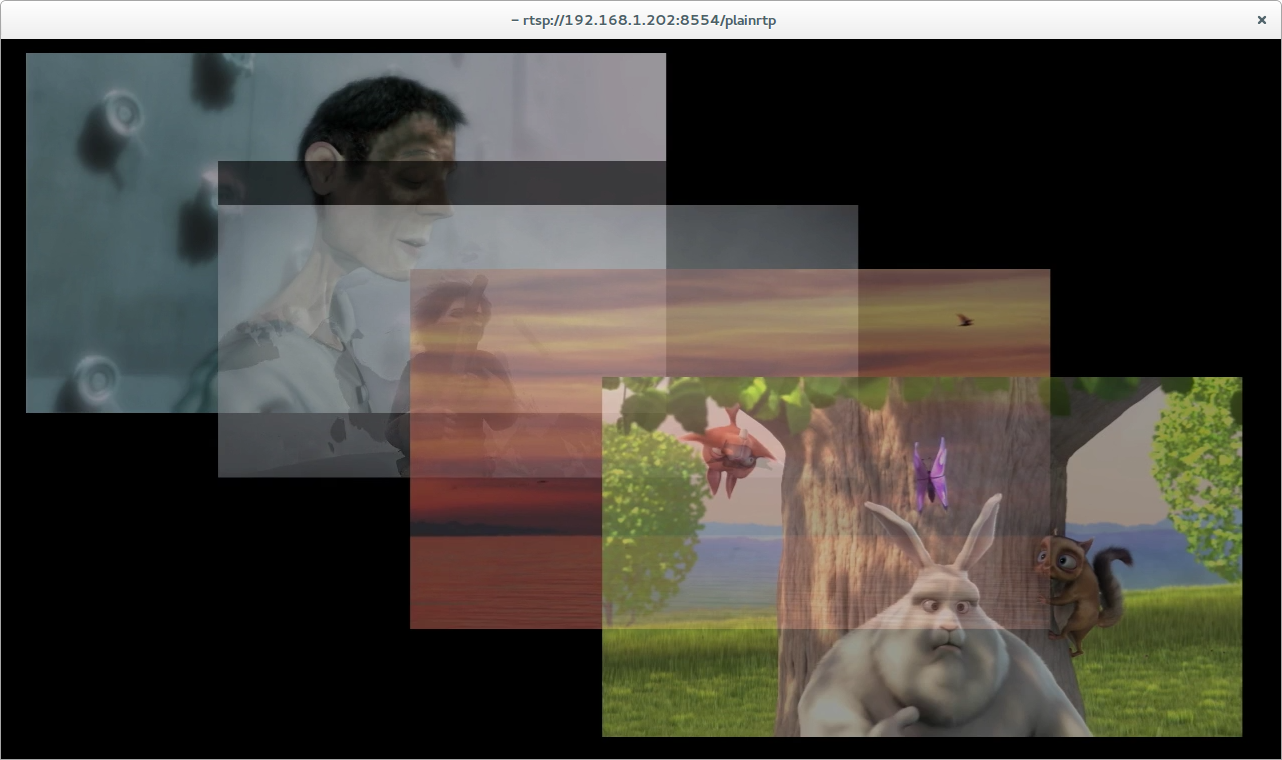
\includegraphics[width=0.90\textwidth]{./images/outAVmix.png}
\caption{Generic scenario - video mixing configuration result}
\label{F:outVMix}
\end{center}
\end{figure}

\vbox{Let us focus now on the results regarding the pipeline performance parameters. The CPU usage of the containerized audio and video mixer obtained by averaging the averages, shown in Figure \ref{F:gsavgcpu}, is 23,02\%.}

\begin{figure}[!htb]
\begin{center}
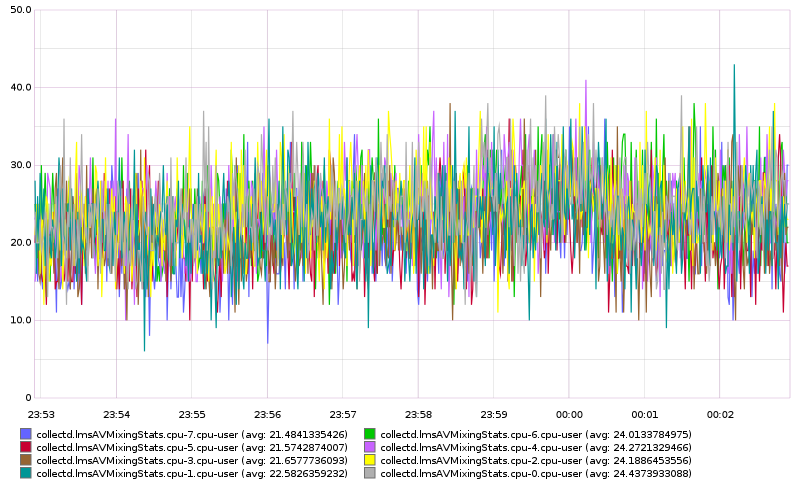
\includegraphics[width=0.90\textwidth]{./images/testAVMix/AVMixCPU.png}
\caption{Generic scenario - average CPU usage}
\label{F:gsavgcpu}
\end{center}
\end{figure}

\vbox{The audio and video average pipeline delay introduced in this scenario is shown in Figure \ref{F:gsavgpt}. There are two path groups, the "recevier to mixer" paths and the "mixer to transmitter" path (see Figure \ref{F:gdsc}).}

\begin{figure}[!htb]
  \begin{center}
    \begin{subfigmatrix}{2}
      \subfigure[Audio paths]
         {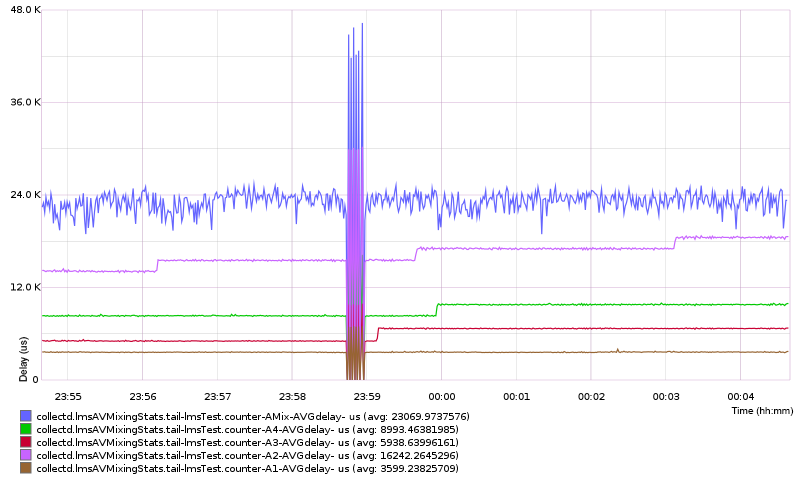
\includegraphics{./images/testAVMix/AVMixAudioAVGdelay.png}\label{SF:S5}} 
      \subfigure[Video paths]
         {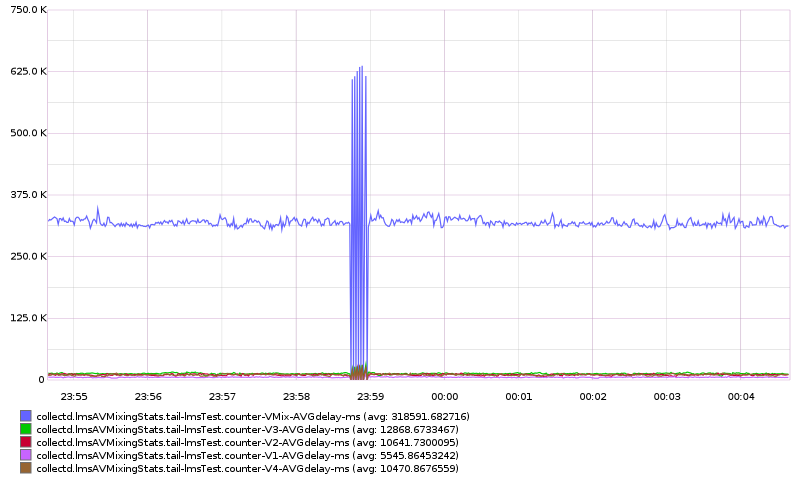
\includegraphics{./images/testAVMix/AVMixVideoAVGdelay.png}\label{SF:S6}} 
    \end{subfigmatrix}
    \caption{Generic scenario - paths average processing time}
    \label{F:gsavgpt}
  \end{center}
\end{figure}

\vbox{The average delay introduced for the audio "receiver to mixer" paths averages is 8,6 milliseconds and the audio "mixer to transmitter" path average delay is 23,1 milliseconds. Then, by adding the maximum average path (16,2 ms), a total average value of 39,3 milliseconds of processing time involving the audio pipeline is achieved. Regarding the pipeline's video path, an average of 9,89 milliseconds is obtained by averaging the "receiver to mixer" video paths average processing times. By adding the average of the "mixer to transmitter" path processing time of 67 milliseconds to the maximum average obtained in the "receiver to mixer" path (12,8 ms) a total average of 79,8 milliseconds of delay introduced for the video pipeline is obtained. Therefore, the generic scenario demonstrates that LMS achieves acceptable processing time values for real-time\footnote{Real-time parameters, in media streaming, mean a total processing time (i.e.: added delay between origin and destination) of 150 to 200 milliseconds} audio-visual media content production.}

\begin{figure}[!htb]
  \begin{center}
    \begin{subfigmatrix}{2}
      \subfigure[Audio paths]
         {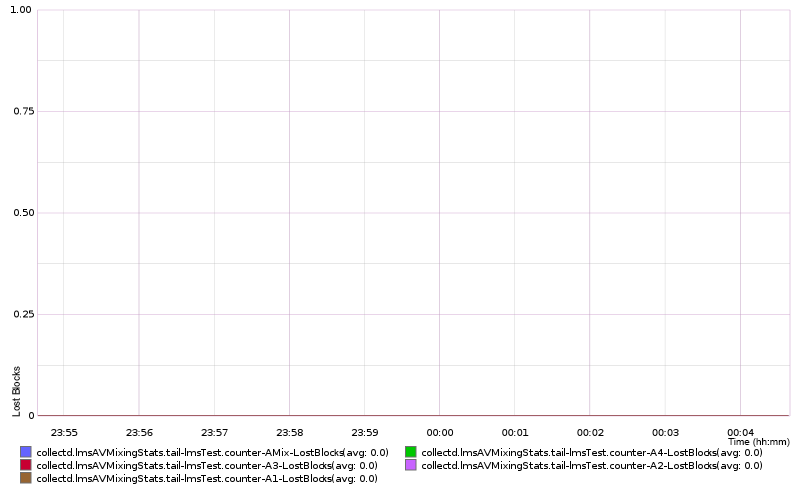
\includegraphics{./images/testAVMix/AVMixAudioLostBlocs.png}\label{SF:S7}} 
      \subfigure[Video paths]
         {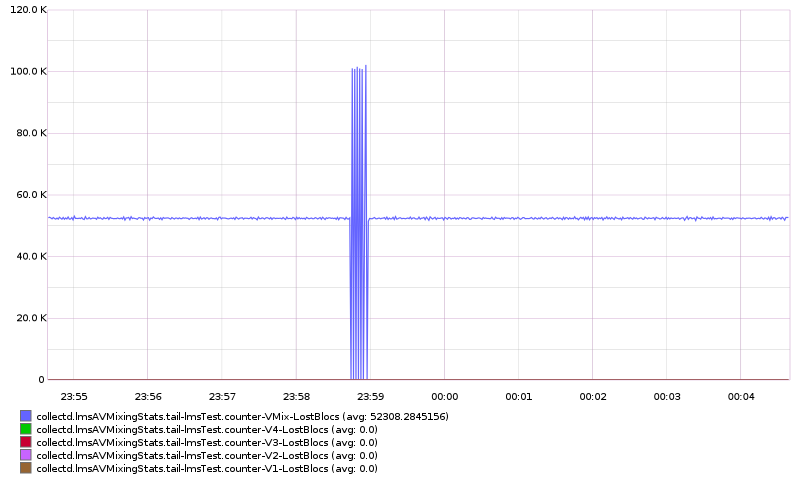
\includegraphics{./images/testAVMix/AVMixVideoLostBlocs.png}\label{SF:S8}} 
    \end{subfigmatrix}
    \caption{Generic scenario - paths accumulated lost blocks}
    \label{F:gsalb}
  \end{center}
\end{figure}

\vbox{Figure \ref{SF:S7} illustrates that the audio paths of the accumulated lost blocks remains to zero, meaning that the audio pipeline is not discarding any data at any filter, which is an important fact because losing any byte of audio would mean noticing some effects (i.e.: audio clips).} 

Then regarding the video "receiver to mixer" paths there aren't accumulated data losses. But, "mixer to transmitter" path reaches around 52.308 lost data blocks. The fact of having lost data blocks is due to the transitory period of the mixer filter. However, this accumulated losses remains constant, meaning that there are no more data blocks lost.

So, although this scenario is being deployed in a i7 processor laptop, it's able to real-time mix four couples of audio and video streams without issues.

Finally, to point out that the signal discontinuities that appear in some figures are due to the fact of transmitting origin streams in a pseudo-live mode, which means audio and video loops. Therefore, this noise appears when the origin streams restart.